\documentclass{exam}
\usepackage[utf8]{inputenc}
\usepackage{lmodern}
\usepackage{microtype}

% \usepackage[parfill]{parskip}
\usepackage[dvipsnames]{xcolor}
\usepackage{amsmath}
\usepackage{amsfonts}
\usepackage{amsthm}
\usepackage{siunitx}
\DeclareSIUnit\year{yr}
\DeclareSIUnit\foot{ft}
\DeclareSIUnit\litre{\liter}

\usepackage{skull}

\usepackage{pgfplots}
\usepgfplotslibrary{polar}
\pgfplotsset{compat=1.11}
\usepgfplotslibrary{statistics}
\usepackage{graphicx}
\usepackage{sidecap}
\sidecaptionvpos{figure}{c}
\usepackage{float}
\usepackage{gensymb}
\usepackage{tkz-euclide}
\usetkzobj{all}
\usepackage{commath}
\usepackage{hyperref}
\usepackage{enumitem}
\usepackage{wasysym}
\usepackage{multicol}
\usepackage{mathtools}
\usepackage{tcolorbox}
\usepackage{tabularx}
\usepackage[version=4]{mhchem}
\usepackage{changepage}
\usepackage{listings}
\lstset{basicstyle=\ttfamily\linespread{0.8}\small}

\renewcommand*{\thefootnote}{\fnsymbol{footnote}}

\newtheorem*{thm}{Theorem}
\newtheorem*{iden}{Identity}
\newtheorem*{lemma}{Lemma}
\newtheorem{obs}{Observation}
\theoremstyle{definition}
\newtheorem*{defn}{Definition}
\newtheorem*{ex}{Example}
\newtheorem{con}{Construction}
\newtheorem*{alg}{Algorithm}

\newtheoremstyle{break}
  {\topsep}{\topsep}%
  {\itshape}{}%
  {\bfseries}{}%
  {\newline}{}%
\theoremstyle{break}
\newtheorem*{bthm}{Theorem}

% russian integral
\usepackage{scalerel}
\DeclareMathOperator*{\rint}{\scalerel*{\rotatebox{17}{$\!\int\!$}}{\int}}

% \DeclareMathOperator*{\rint}{\int}

\pgfplotsset{vasymptote/.style={
    before end axis/.append code={
        \draw[densely dashed] ({rel axis cs:0,0} -| {axis cs:#1,0})
        -- ({rel axis cs:0,1} -| {axis cs:#1,0});
    }
}}

% \pointsinrightmargin
\boxedpoints
\pointname{}

\newcommand{\questioA}{\question[\texttt{\textbf{\color{Cerulean} A}}]}
\newcommand{\questioM}{\question[\texttt{\textbf{\color{PineGreen} M}}]}
\newcommand{\questioE}{\question[\texttt{\textbf{\color{WildStrawberry} E}}]}
\newcommand{\questioS}{\question[\texttt{\textbf{\color{Goldenrod} S}}]}
\newcommand{\questioO}{\question[\texttt{\textbf{\color{BurntOrange} O}}]}

\newcommand{\parA}{\part[\texttt{\textbf{\color{Cerulean} A}}]}
\newcommand{\parM}{\part[\texttt{\textbf{\color{PineGreen} M}}]}
\newcommand{\parE}{\part[\texttt{\textbf{\color{WildStrawberry} E}}]}
\newcommand{\parS}{\part[\texttt{\textbf{\color{Goldenrod} S}}]}
\newcommand{\parO}{\part[\texttt{\textbf{\color{BurntOrange} O}}]}

\newcommand{\subparA}{\subpart[\texttt{\textbf{\color{Cerulean} A}}]}
\newcommand{\subparM}{\subpart[\texttt{\textbf{\color{PineGreen} M}}]}
\newcommand{\subparE}{\subpart[\texttt{\textbf{\color{WildStrawberry} E}}]}
\newcommand{\subparS}{\subpart[\texttt{\textbf{\color{Goldenrod} S}}]}
\newcommand{\subparO}{\subpart[\texttt{\textbf{\color{BurntOrange} O}}]}

\newcommand{\mainHeader}[2]{\section*{NCEA Level 2 Mathematics\\#1. #2}}
\newcommand{\mainHeaderHw}[2]{\section*{NCEA Level 2 Mathematics (Homework)\\#1. #2}}
\newcommand{\seealso}[1]{\begin{center}\emph{See also #1.}\end{center}}
\newcommand{\drills}[1]{\begin{center}\emph{Drill problems: #1.}\end{center}}
\newcommand{\basedon}[1]{\begin{center}\emph{Notes largely based on #1.}\end{center}}


\begin{document}

\mainHeader{19}{The Statistical Enquiry Process}
Statistics is one of the most important tools in experimental science, and medicine. Even in the everyday world we are
bombarded with statistics given to us by the media, politicians, and the internet. Because of this, being able to interpret
statistics and judging whether or not they support a given argument, result, or point of view is an important skill in
the modern world.

\begin{center}
  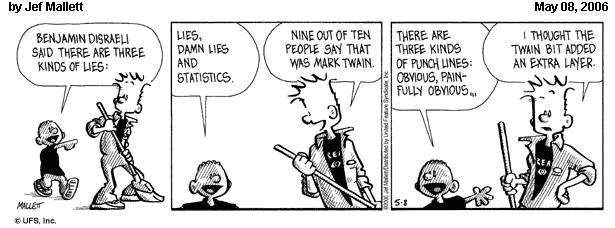
\includegraphics[width=0.7\textwidth]{stats}
\end{center}

The statistical inquiry cycle is something you should already know about from as far back as intermediate school.

\begin{enumerate}
  \item We begin with a question we want to answer, and perhaps a hypothesis backed up by some theory.
  \item We decide what data we need to collect to answer our question.
  \item We plan how we will collect our data, and how we will ensure it is accurate and precise.
  \item We plan how we will process our data.
  \item We collect our data. (This is intentionally \emph{after} we plan how we will use it.)
  \item We process our data in accordance with our plan.
  \item We answer our question.
  \item We decide how reliable our process was.
  \item We write a report, detailing \emph{all} of the above steps, such that another person
        could pick it up and try to replicate our findings.
\end{enumerate}

\subsection*{Writing a question, and deciding on data to collect}
A question should be written clearly and precisely, and there should be a straightforward way to answer it.

Some good questions:
\begin{itemize}
  \item Are high school students in Wellington City more likely to cycle to school than students in Upper Hutt?
  \item Do male Y12 students tend to be taller than female Y12 students?
  \item Does this drug lower the risk of heart failure after a stroke?
  \item With what speed does a \SI{0.5}{\kilo\gram} weight hit the ground after being dropped \SI{10}{\metre}?
\end{itemize}

Some bad questions (why?):
\begin{itemize}
  \item Does this drug work?
  \item Will I crash if I drink and drive?
  \item Does the average person support the attempt by the USA to bring freedom and democracy to other places in the world?
  \item Any question you write after you've already collected your data!\footnote{Try googling `data dredging': ``Data dredging (also data fishing, data snooping,
        data butchery, and p-hacking) is the misuse of data analysis to find patterns in data that can be presented as statistically significant when in fact there
        is no real underlying effect. This is done by performing many statistical tests on the data and only paying attention to those that come back with
        significant results, instead of stating a single hypothesis about an underlying effect before the analysis and then conducting a single test for it.

        ``The process of data dredging involves automatically testing huge numbers of hypotheses about a single data set by exhaustively searching—perhaps for
        combinations of variables that might show a correlation, and perhaps for groups of cases or observations that show differences in their mean or in
        their breakdown by some other variable.'' (Wikipedia contributors. (2019, January 13). Data dredging. In Wikipedia, The Free Encyclopedia. Retrieved 22:29, January 20, 2019, from \url{https://en.wikipedia.org/w/index.php?title=Data_dredging&oldid=878260765})}
\end{itemize}

When you write your question, you should come up with a good idea as to what kind of data you will need to gather to answer it. This could
be something like a set of measurements, or responses to a questionnaire, or something else.

\subsection*{Planning how to collect data}
Usually, we want to collect data to answer a question about a whole population. Unfortunately, it's not cheap or easy to measure or survey
every individual in a population, so we have to make do with examining a smaller sample; we then need to process our data to make an educated
inference about the state of the full population. In order to do this, we need a reliable sample that reflects the trends in the population.

In general, we need two things from a sample:
\begin{itemize}
  \item A sample needs to be \emph{large}.
  \item A sample needs to be \emph{random}.
\end{itemize}

Both of these statements are harder to unpack than they might seem right now:- they are what we will
discuss in the next topic.

At this stage, we also decide how we are going to actually collect the data: will we need to write a questionnaire? Do we need
any specialised equipment? How are we going to ensure the accuracy and precision of our data? Do we need a control group?

\subsection*{Planning how to process data}
We then need to decide what we are going to do to our massive spreadsheet of data after we collect it. If we want to work
out the average value of some measurement, we need to decide how to do this (median, or mean, or something else?). If we
want to work out whether there is a difference in some value between two populations (whether one group is taller than
another group, for example), then we need to decide how big a difference will be `significant' and not likely to be due
to random chance.

\subsection*{Collecting and processing the data}
This is where we apply the plan we've come up with so far. If we deviate from the plan in any way, we carefully specify
why and how we are doing so, and we make a careful note that this needs to be stated in our report. Further, we \emph{only}
peform the analysis we planned to do. (This is for two reasons: firstly, as I mentioned above, if you measure a bunch of
variables then some of them will end up significant simply due to random chance; and secondly, the data we planned to
collect is more likely to be reliable than the data we collected along the way with no planning.)

\subsection*{Answering the question}
Now, we look at our data processing and we give a simple answer to our question together with a rough idea of how likely
we are to be correct:

\begin{center}\itshape
  According to our analysis, our hypothesis was incorrect: in our sample, girls tended to be taller than boys. We found
  that the mean height of the girls in our sample was \SI{1.8}{\metre}, while the mean height of the boys was \SI{1.6}{\metre}.
  The difference between these means is large enough that it is unlikely to be due to random chance, and so it is likely that
  in the general population of the class the average height of girls is greater than the average height of boys.
\end{center}

\subsection*{Evaluating our process}
The final step we perform before writing down our report is to evaluate our findings.
\begin{itemize}
  \item What difficulties did we encounter when trying to measure our results?
  \item Did we have to change any of our planning while performing our experiment?
  \item Did anything go wrong that might affect our results?
  \item Is there anything we would do differently? Why?
\end{itemize}

Why do we do this? Because it allows people who read our report to decide for themselves how reliable our process
and results are, and it allows people who want to reproduce our findings to be aware of why we chose to do things
a particular way and what challenges we faced when performing our experiment.

\subsection*{Questions}
This week, we will work through the planning for a sample task provided by the Ministry of Education (resource 2.10A).

It has been claimed that teenagers are becoming addicted to energy drinks (which contain high amounts of caffeine) without
knowledge of the short-term or long-term effects. People are also concerned that teenagers feel the need for mind or
body-altering substances like energy drinks (see the web links below).

\begin{itemize}
  \item \url{http://www.stuff.co.nz/the-press/news/2820097/Caffeine-drinks-may-be-hurting-teenagers}
  \item \url{http://kidshealth.org/teen/food_fitness/nutrition/caffeine.html}
  \item \url{http://www.foodsafety.govt.nz/elibrary/industry/Caffeine_Intake-Confirms_Advice.htm}.
\end{itemize}
In a group, use the information on caffeine, Resource 1, and select an experimental situation, based on the effects of drinking
caffeine, to investigate. Identify the variables you think are important, and write a question to investigate.

The following situations are suggested as a basis for your experiment:
\begin{itemize}
  \item the effect of drinking caffeine on heart rate;
  \item the effect of drinking caffeine on reaction times;
  \item the effect of drinking caffeine on memory.
\end{itemize}

Write a plan for the experiment. The plan should:
\begin{itemize}
  \item describe the variables and measures you have chosen and why you have chosen them;
  \item explain how you will collect your data and record your results;
  \item link to relevant knowledge about the situation;
  \item describe any related variables and the possible effects of these;
  \item describe the experimental method.
\end{itemize}

\end{document}

